\documentclass[11pt,a4paper]{article}

% ---------- packages ----------
\usepackage[margin=2.2cm]{geometry}
\usepackage{fontspec}
\usepackage{graphicx}
\usepackage{booktabs}
\usepackage{longtable}
\usepackage{tabularx}
\usepackage{array}
\usepackage{enumitem}
\usepackage{xcolor}
\usepackage{titlesec}
\usepackage{float}
\usepackage{caption}
\usepackage[hidelinks]{hyperref}

\definecolor{gblue}{HTML}{1A73E8}
\definecolor{ggray}{HTML}{5F6368}
\hypersetup{colorlinks=true, urlcolor=gblue, linkcolor=black}

\titleformat{\section}{\Large\bfseries\color{gblue}}{\thesection.}{0.5em}{}
\titleformat{\subsection}{\large\bfseries}{\thesubsection}{0.5em}{}
\titlespacing*{\section}{0pt}{1.2em}{0.5em}
\titlespacing*{\subsection}{0pt}{0.9em}{0.35em}

\setlength{\parindent}{0pt}
\setlength{\parskip}{0.5em}
\setlist{itemsep=0.15em, topsep=0.3em}
\renewcommand{\arraystretch}{1.25}
\captionsetup{font=small, labelfont=bf}

\newcommand{\code}[1]{\texttt{#1}}
\newcolumntype{L}[1]{>{\raggedright\arraybackslash}p{#1}}
\newcolumntype{Y}{>{\raggedright\arraybackslash}X}

% ---------- document ----------
\begin{document}

\begin{center}
  {\LARGE\bfseries\color{gblue} CMPE 48A Term Project -- Phase 1 Report\par}
  \vspace{0.4em}
  {\large Cloud-Native Deployment of \emph{Local History Story Map} on Google Cloud Platform\par}
  \vspace{0.3em}
  {\color{ggray} November 2026\par}
  \vspace{0.3em}
  {\color{gblue}\rule{\linewidth}{1pt}}
\end{center}

% ------------------------------------------------------------
\section{Team}

\begin{tabularx}{\linewidth}{L{5cm}Y}
\toprule
\textbf{Role} & \textbf{Name} \\
\midrule
Developer & Aysu Keskin \\
Developer & \textbf{[Partner Name]} \\
\bottomrule
\end{tabularx}

% ------------------------------------------------------------
\section{Application Code}

\textbf{Repository:} \url{https://github.com/AysuKeskin/storymap-cloud-native}

The application is \emph{Local History Story Map}, a platform where users
discover and publish location-based community stories through a map, a feed,
a timeline and full-text search. We reuse the application code that was
developed earlier in the CMPE~354 software-engineering course (original
upstream: \url{https://github.com/bounswe/bounswe2026group4}). The cloud-native
design, the Kubernetes manifests, Terraform code, Cloud Functions and Locust
tests are new work for this course.

\begin{tabularx}{\linewidth}{L{4.2cm}Y}
\toprule
\textbf{Layer} & \textbf{Technology} \\
\midrule
Backend API & Django 4.2 + Django REST Framework, Gunicorn, JWT auth \\
Web frontend & React + Vite, served by nginx \\
Mobile client & Expo / React Native (consumes the same API) \\
Database & MySQL 8.0 \\
Already containerised & Dockerfiles for backend and nginx/frontend, Docker Compose \\
\bottomrule
\end{tabularx}

Main API domains: users and authentication, stories (map / feed / timeline /
search), media uploads, comments and likes, tags, notifications, gamification
(badges) and a geocoding proxy to OpenStreetMap Nominatim.

\textbf{Changes planned to make the application cloud-native}
\begin{enumerate}
  \item Move media storage from the local disk to \textbf{Cloud Storage} with
        \code{django-storages}, so that API pods are stateless and can be
        scaled freely.
  \item Replace the per-process in-memory cache with a shared \textbf{Redis}
        cache. This also gives a distributed rate-limit lock for the Nominatim
        proxy, which today works only within one process.
  \item Move e-mail sending out of the request path. The API publishes an event
        to \textbf{Pub/Sub} and a \textbf{Cloud Function} sends the e-mail.
  \item Add \textbf{image thumbnail generation} as a Cloud Function triggered
        by uploads to the bucket.
  \item Read all configuration from Kubernetes Secrets and ConfigMaps, and run
        database migrations as a Kubernetes \code{Job}.
\end{enumerate}

% ------------------------------------------------------------
\section{Tentative Cloud Architecture}

\begin{figure}[H]
  \centering
  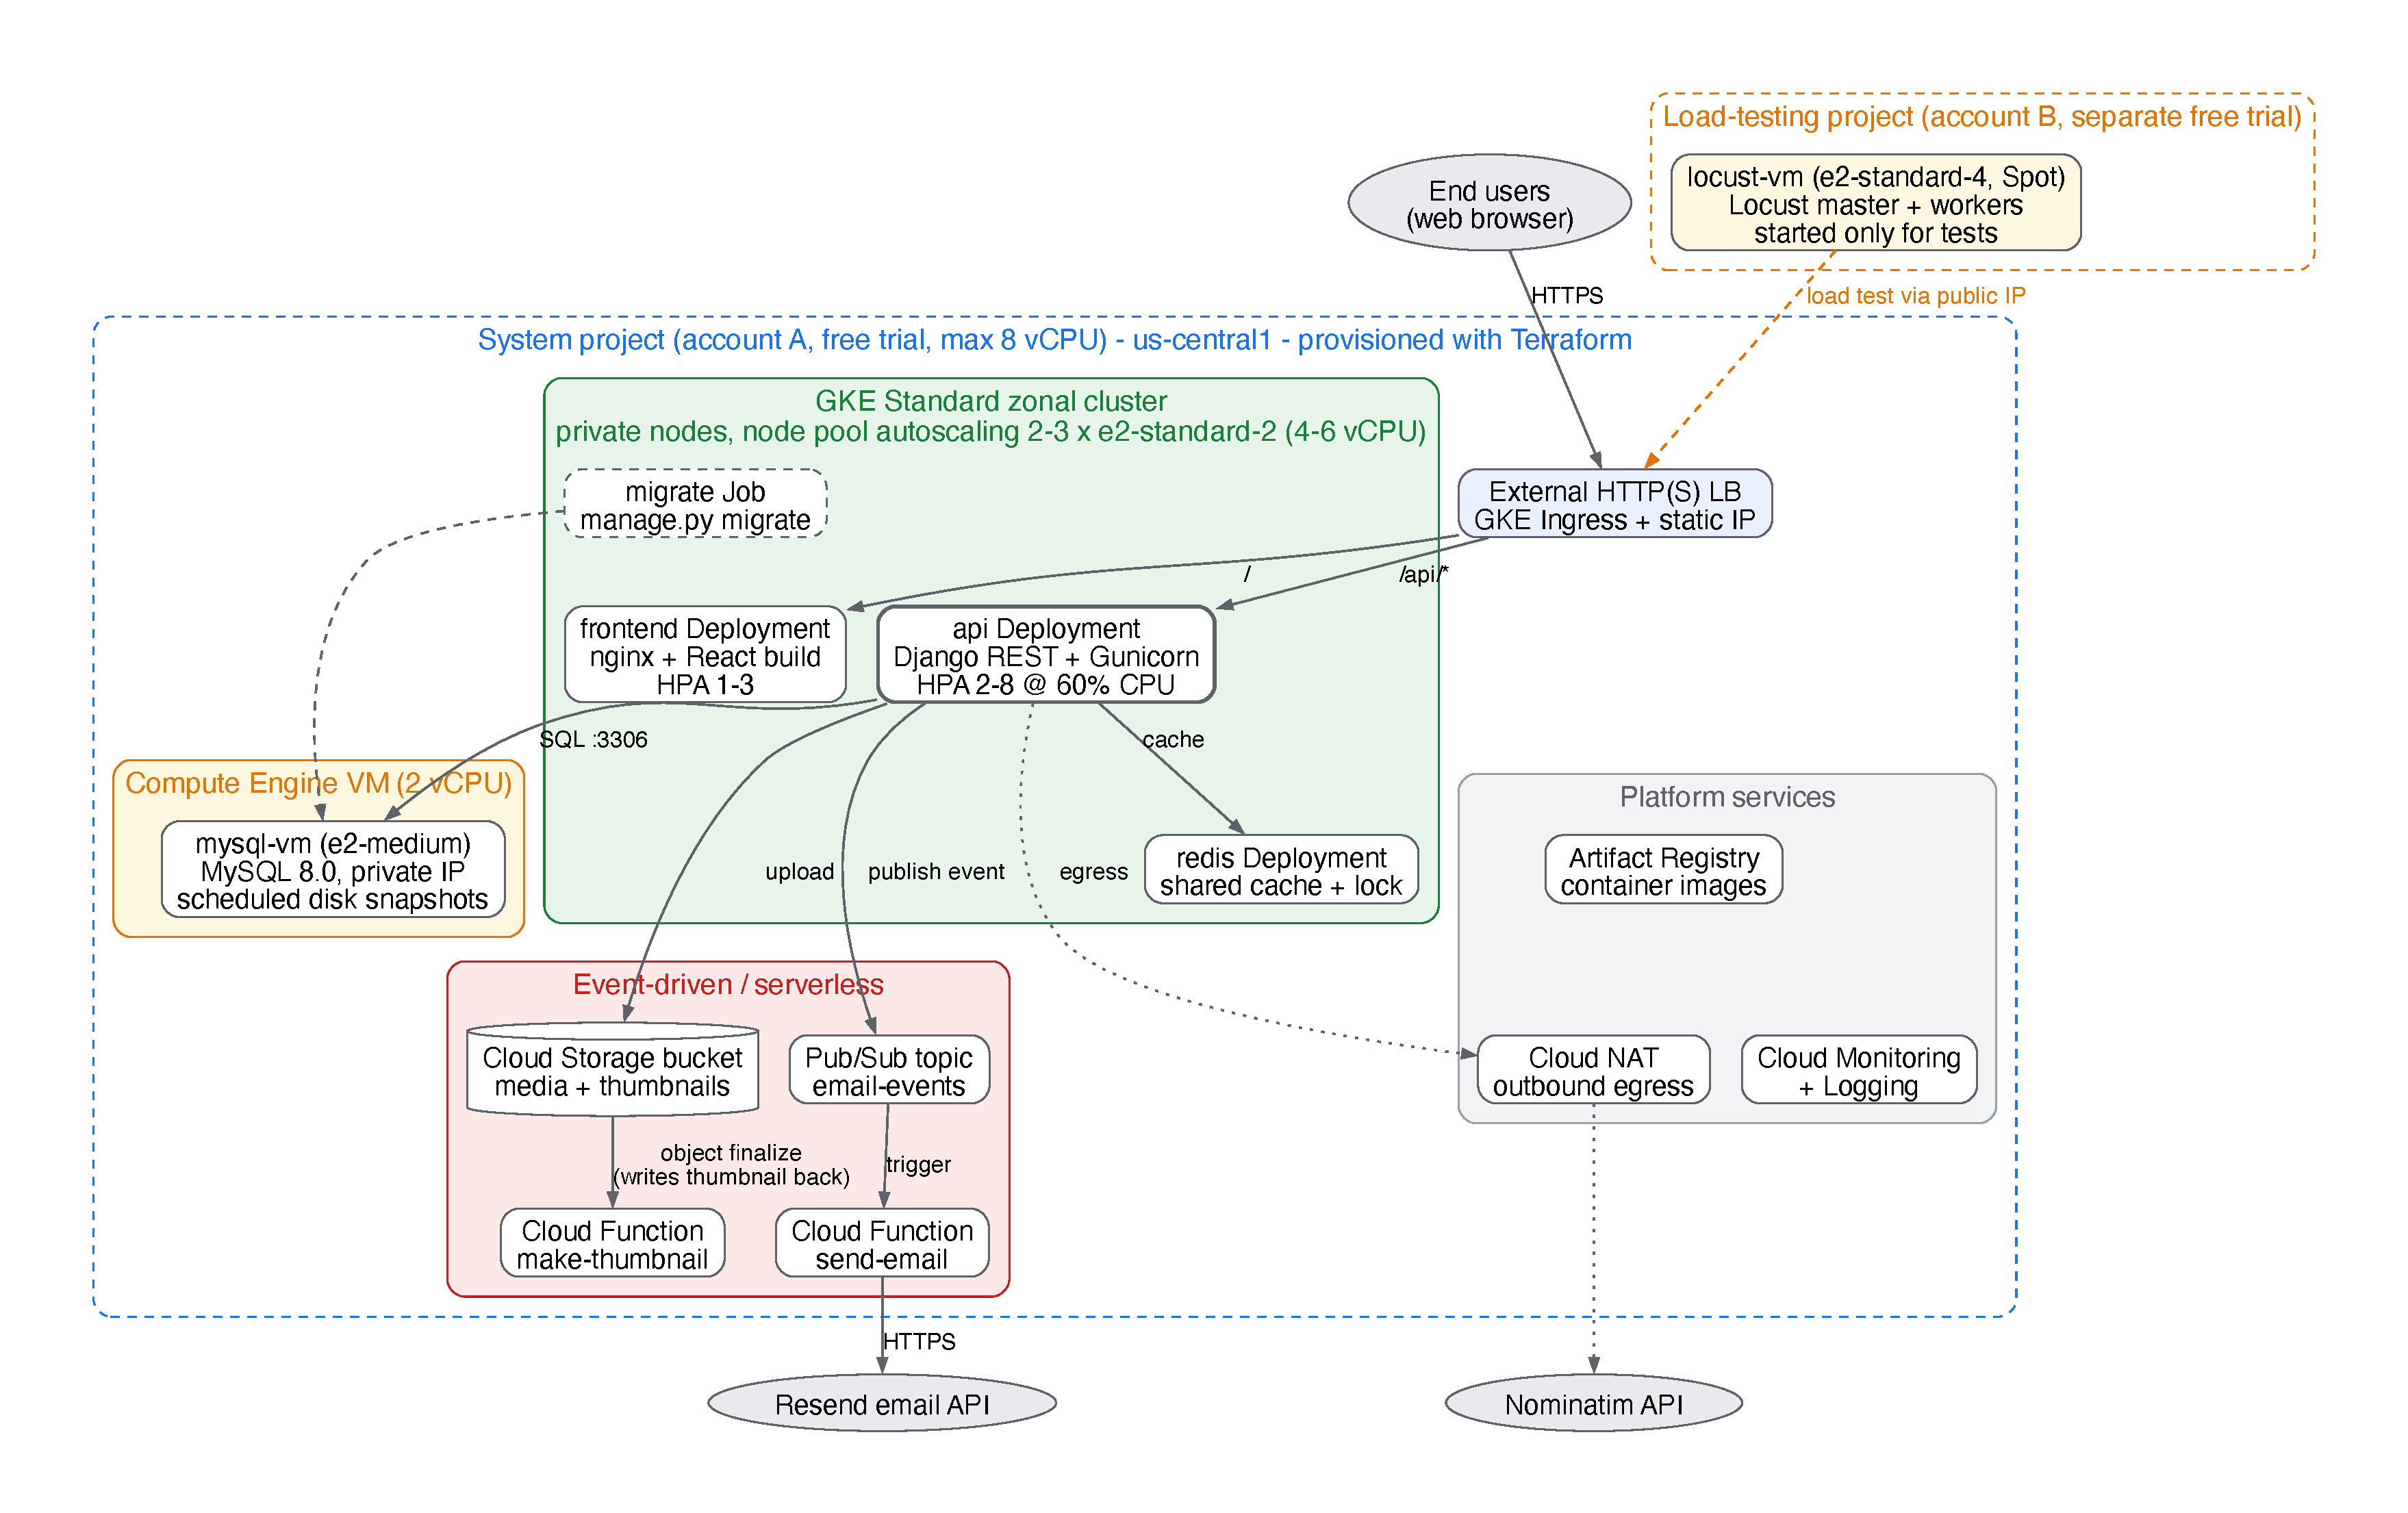
\includegraphics[width=\linewidth]{architecture.pdf}
  \caption{Tentative GCP architecture. All resources are provisioned with Terraform.}
  \label{fig:arch}
\end{figure}

\subsection{Components}

{\small
\begin{longtable}{L{3.1cm}L{4.3cm}L{7.6cm}}
\toprule
\textbf{Component} & \textbf{GCP service} & \textbf{Role in the system} \\
\midrule
\endfirsthead
\toprule
\textbf{Component} & \textbf{GCP service} & \textbf{Role in the system} \\
\midrule
\endhead
\bottomrule
\endfoot
\textbf{Load balancer} & External HTTP(S) LB (created by GKE Ingress), static IP &
  Single public entry point. Routes \code{/api/*} to the API service and
  \code{/} to the frontend. \\
\textbf{frontend} & GKE Deployment (+ HPA 1--3) &
  nginx serving the compiled React app. Lightweight and stateless. \\
\textbf{api} & GKE Deployment (+ HPA 2--10 at 60\,\% CPU) &
  Django REST API on Gunicorn. Main scaling target and the focus of the
  performance tests. \\
\textbf{redis} & GKE Deployment + ClusterIP Service &
  Shared cache for hot read endpoints (\code{/stories/map},
  \code{/stories/feed}, \code{/stories/timeline}), geocoding results and a
  distributed lock. Runs in-cluster instead of Memorystore to save budget. \\
\textbf{migrate} & Kubernetes Job &
  Runs \code{manage.py migrate} before each rollout. \\
\textbf{mysql-vm} & Compute Engine VM (e2-medium) &
  MySQL 8.0 on a private IP, reachable only from inside the VPC. Persistent
  disk with a scheduled snapshot policy. Chosen over Cloud SQL for cost and to
  satisfy the VM requirement with a stateful, functional role. \\
\textbf{locust-vm} & Compute Engine VM (e2-standard-4) &
  Runs Locust master and workers. Started only during experiments so that load
  is generated outside the cluster it is measuring. \\
\textbf{Media bucket} & Cloud Storage &
  Stores user-uploaded images, audio and video, plus generated thumbnails. \\
\textbf{make-thumbnail} & Cloud Function (2nd gen), GCS \emph{object finalize} trigger &
  Creates resized thumbnails for every uploaded image and writes them back to
  the bucket. \\
\textbf{email-events} & Pub/Sub topic &
  Asynchronous queue that decouples the API from e-mail delivery (registration
  verification, password reset, notification e-mails). \\
\textbf{send-email} & Cloud Function (2nd gen), Pub/Sub trigger &
  Consumes \code{email-events} and sends the message through the Resend e-mail
  API. Retries on failure. \\
\textbf{Artifact Registry} & Docker repository &
  Stores the \code{api} and \code{frontend} images built by GitHub Actions. \\
\textbf{Cloud NAT} & Cloud Router + NAT &
  Outbound internet access for private GKE nodes and VMs (Nominatim, package
  installs). Nothing in the VPC has a public IP. \\
\textbf{Monitoring / Logging} & Cloud Monitoring, Cloud Logging &
  CPU, memory, pod count, LB latency and error metrics used in the performance
  evaluation. \\
\end{longtable}
}

\subsection{Interactions}

\begin{enumerate}
  \item \textbf{Read path.} A request goes Client $\rightarrow$ LB
        $\rightarrow$ \code{api} pod. The pod checks Redis first. On a cache
        miss it queries MySQL on the VM and stores the result in Redis with a
        short TTL.
  \item \textbf{Write path (story with media).} The \code{api} pod writes the
        story row to MySQL and streams the file to Cloud Storage. The bucket's
        \emph{finalize} event triggers \code{make-thumbnail}, which writes the
        thumbnail next to the original.
  \item \textbf{Asynchronous e-mail.} Registration and notification flows
        publish a small JSON message to \code{email-events} and return
        immediately. \code{send-email} then delivers the message. A slow
        e-mail provider no longer slows down API requests.
  \item \textbf{Scaling.} The HPA adds \code{api} pods when average CPU
        exceeds 60\,\%. The GKE cluster autoscaler adds nodes (2 $\rightarrow$
        5) when pods cannot be scheduled.
  \item \textbf{Deployment.} Terraform creates the VPC, NAT, GKE cluster, VMs,
        bucket, Pub/Sub topic, Cloud Functions, Artifact Registry and a
        billing budget. Kubernetes manifests (Deployments, Services, HPA,
        Ingress, Job) are then applied with \code{kubectl}.
\end{enumerate}

\subsection{Planned performance experiments (preview)}

Locust user classes will simulate (a) anonymous visitors browsing the map,
feed and story details, (b) logged-in users who like and comment, and
(c) content creators who post stories with images.

\begin{tabularx}{\linewidth}{YY}
\toprule
\textbf{Independent variables} & \textbf{Dependent variables} \\
\midrule
Number of concurrent users and spawn rate & p50 / p95 / p99 latency \\
Read vs.\ write traffic mix & Throughput (requests per second) \\
Redis cache on vs.\ off & Error rate \\
HPA on (2--10 pods) vs.\ fixed replicas & CPU and memory of pods and the MySQL VM \\
Synchronous vs.\ Pub/Sub e-mail & Pod and node count over time \\
\bottomrule
\end{tabularx}

% ------------------------------------------------------------
\section{Cost Estimation}

Prices are \textbf{list prices for \code{us-central1}} taken from the GCP
pricing pages. They will be re-checked in the GCP Pricing Calculator before
deployment. We assume about \textbf{two months} of usage (mid-November to
mid-January).

\subsection{Monthly baseline (system running 24/7)}

{\small
\begin{longtable}{L{3.6cm}L{3.9cm}L{3.6cm}L{3.4cm}}
\toprule
\textbf{Resource} & \textbf{Configuration} & \textbf{Unit price} & \textbf{Monthly cost} \\
\midrule
\endfirsthead
\toprule
\textbf{Resource} & \textbf{Configuration} & \textbf{Unit price} & \textbf{Monthly cost} \\
\midrule
\endhead
GKE management fee & 1 zonal Standard cluster & \$0.10/h ($\approx$\,\$73) &
  \textbf{\$0.00} (covered by the \$74.40/month GKE free-tier credit) \\
GKE nodes & 2 $\times$ e2-medium (2 vCPU, 4\,GB) & \$0.0335/h each & \$48.92 \\
Node boot disks & 2 $\times$ 30\,GB pd-standard & \$0.04/GB-month & \$2.40 \\
mysql-vm & 1 $\times$ e2-medium & \$0.0335/h & \$24.46 \\
mysql-vm disk + snapshots & 20\,GB pd-balanced + $\sim$5\,GB snapshots & \$0.10 and \$0.05/GB-month & \$2.25 \\
HTTP(S) Load Balancer & 1 forwarding rule & \$0.025/h & \$18.25 \\
Cloud NAT & 3 VM endpoints + low traffic & \$0.0014/h per VM + \$0.045/GB & \$3.57 \\
Cloud Storage & $\sim$2\,GB Standard & \$0.020/GB-month & \$0.04 \\
Artifact Registry & $\sim$2\,GB images (0.5\,GB free) & \$0.10/GB-month & \$0.15 \\
Cloud Functions (2nd gen) & $<$\,100k invocations/month & free tier: 2M req., 180k vCPU-s & \$0.00 \\
Pub/Sub & $<$\,1\,GB/month & first 10\,GiB free & \$0.00 \\
Monitoring and Logging & within free allotment (50\,GiB logs) & -- & \$0.00 \\
Internet egress & $\sim$5--10\,GB & $\sim$\$0.12/GB & $\sim$\$1.00 \\
\midrule
\textbf{Total per month} & & & \textbf{$\approx$\,\$101} \\
\bottomrule
\end{longtable}
}

\subsection{Load-testing campaign (one-off, about 30 test hours)}

{\small
\begin{tabularx}{\linewidth}{L{5.2cm}Y L{2cm}}
\toprule
\textbf{Resource} & \textbf{Usage} & \textbf{Cost} \\
\midrule
locust-vm (e2-standard-4) & 30\,h $\times$ \$0.134/h + 20\,GB disk & \$4.82 \\
Extra GKE nodes from autoscaling & up to 3 $\times$ e2-medium $\times$ 30\,h & \$3.02 \\
LB data processing and egress & $\sim$50\,GB $\times$ \$0.008/GB + misc. & \$1.50 \\
Cloud Functions / Pub/Sub under load & still within the free tier & \$0.00 \\
\midrule
\textbf{Total} & & \textbf{$\approx$\,\$9.50} \\
\bottomrule
\end{tabularx}
}

\subsection{Project total vs.\ the \$300 credit}

{\small
\begin{tabularx}{\linewidth}{L{4.6cm}Y L{2.2cm}L{2.2cm}}
\toprule
\textbf{Scenario} & \textbf{Calculation} & \textbf{Total} & \textbf{Share of \$300} \\
\midrule
Worst case: always on & 2 $\times$ \$101 + \$9.50 & \textbf{$\approx$\,\$212} & 71\,\% \\
Planned: shut down when idle & baseline $\sim$50\,\% of the time + tests & \textbf{$\approx$\,\$110--120} & $\sim$40\,\% \\
\bottomrule
\end{tabularx}
}

\textbf{Cost-control measures}
\begin{itemize}
  \item \code{terraform destroy}, or scaling the node pool to 0 and stopping
        \code{mysql-vm} when the system is not needed. Everything can be
        recreated from code in about 15 minutes.
  \item \code{locust-vm} runs only during experiments and can use
        \textbf{Spot} pricing ($\sim$60--90\,\% cheaper).
  \item Small e2 machine types and 30\,GB pd-standard boot disks instead of the
        100\,GB default.
  \item Redis and MySQL are self-hosted, which avoids Memorystore
        ($\sim$\$35+/month) and Cloud SQL ($\sim$\$25--50/month).
  \item A \textbf{billing budget with alerts at 50\,\%, 75\,\% and 90\,\%} of
        \$300 is created by Terraform (\code{google\_billing\_budget}).
\end{itemize}

\end{document}
